\section{Unknown Unknowns}
\label{sec:unknowns}

In order to provide a detailed discussion of unknown unknowns in the context of a predictive model, it is first necessary to formalize the concepts we will be discussing. Let $x$ represent an example belonging to some problem space $X$. In classification settings, $x$ has a ``true'' label, $\bar{y}$ from some set of possible labels $Y$. The task of a classification is to construct some predictive model, $f(x)$, that can estimate a label for each incoming example ($y = f(x)$) such that the estimated label $y$ mirrors the (usually hidden) true label, $\bar{y}$, as closely as possible. There is a cost $c_{ij}$ for a misclassification decision, when we classify an example from the true category $\bar{y}=y_i$ into a category $f(x)=y_j$. In this work, we are concerned only with models that output a posterior probability estimate over the set of available labels, that is, $f(x) = p(y | x) = \langle p_1, \ldots, p_n \rangle$; such models, through the probability estimates, effectively also  report the estimated misclassification cost of each example:

\begin{eqnarray}
\widehat{\mathit{ExpCost}}(x) =  \sum_{i,j} p_i \cdot p_j \cdot c_{ij} & ~ & \widehat{\mathit{MinCost}}(x) =  \mbox{min}_j \sum_{i} p_i \cdot c_{ij} \label{equ:expcost} 
 \label{equ:mincost}
\end{eqnarray}

Such probabilities can then be used to select a preferred label, for instance by choosing the $y$ with the highest probability, or in the cost-sensitive setting, choosing the label with the least expected cost~\cite{elkan:2001cost}. Note that the focus on models that produce probability estimates is without loss of generality--- there exists a variety of techniques for transforming ``hard-labeling'' models into probability estimators (see, eg.~\cite{domingos1999metacost}).

Notice that Equation~\ref{equ:expcost} provides \emph{estimates} of the misclassification cost. The \emph{actual} misclassification cost can be different and depends on the accuracy of the model and the generated posterior probability estimates. The difference between the estimated and the 
actual misclassification costs gives birth to four different classification scenarios, as depicted in Figure~\ref{fig:quadrant}.

\begin{figure}[t]
\centering
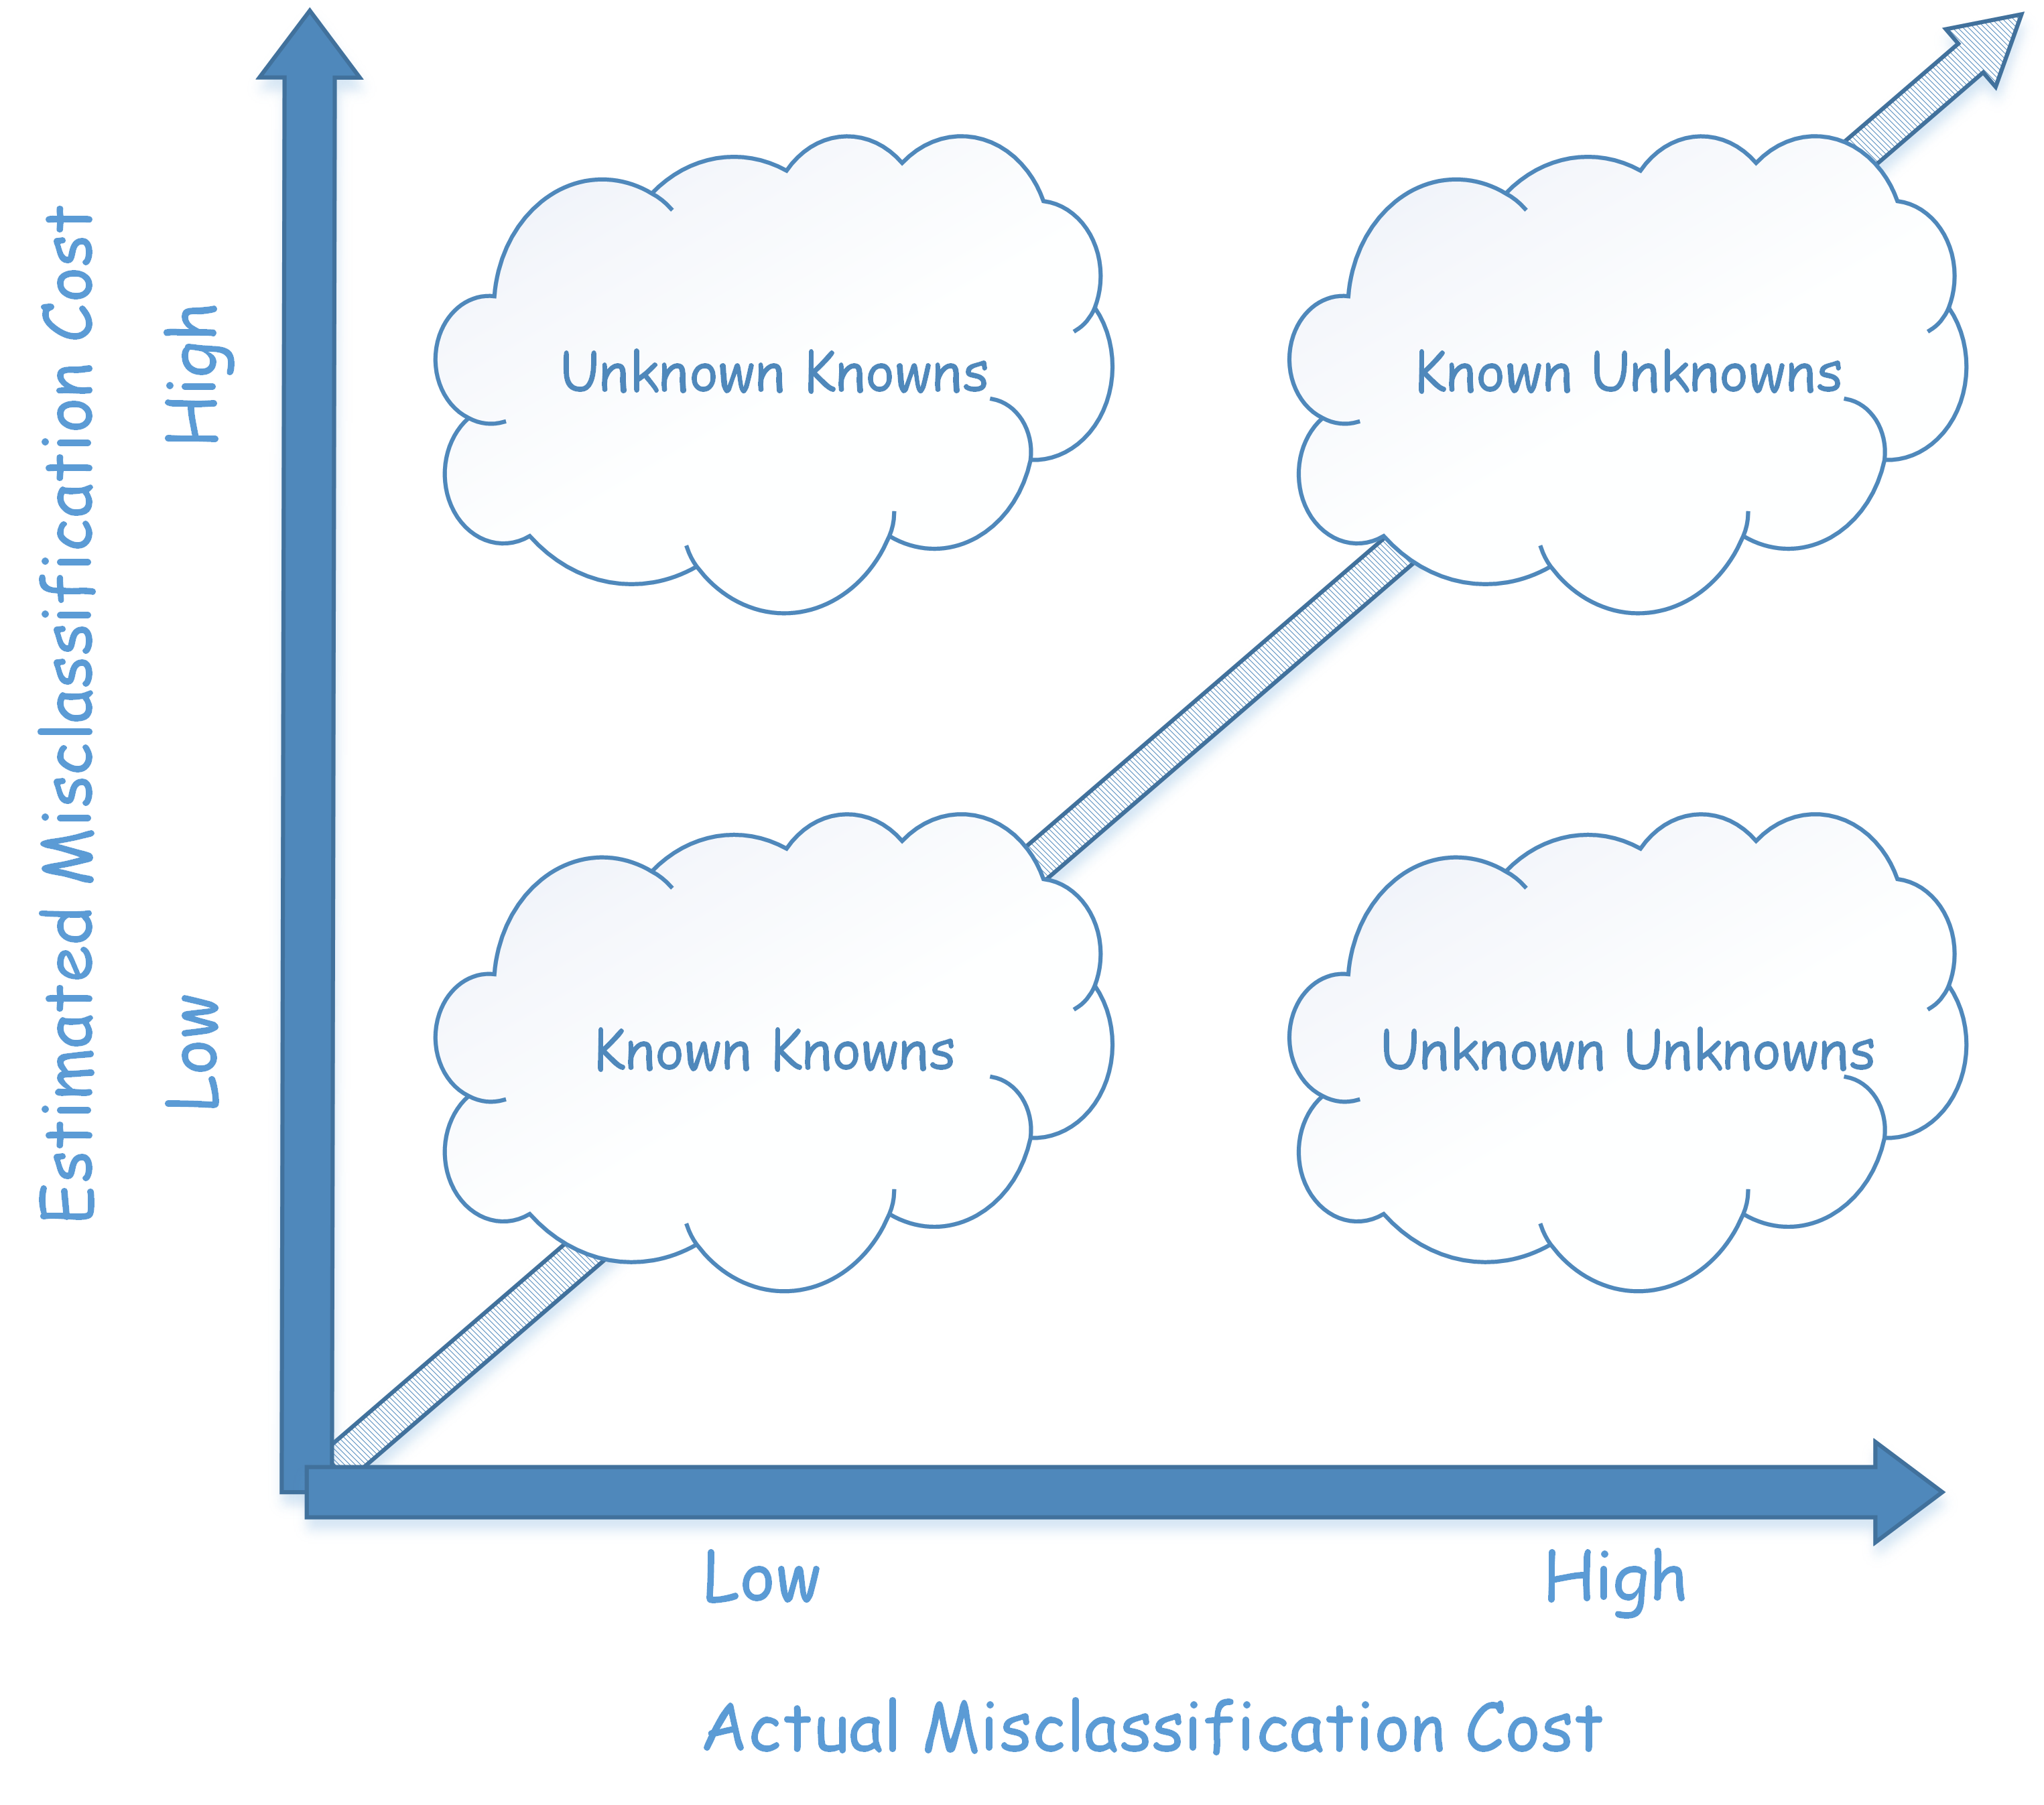
\includegraphics[width=0.5\columnwidth]{plots/Quadrant.png}
\caption{The decisions made by a predictive model can be broadly separated into four conceptual regions: (i)~The ``known knowns,'' which are the examples for which the model is mostly correct and is also confident of being correct; (ii)~The ``known unknowns,'' which are the examples for which the model is often mistaken but also anticipates these mistakes by placing low confidence in the decisions; (iii)~The ``unknown knowns,'' which are the examples for which the model is often correct but returns very low levels of confidence; and (iv)~The ``unknown uknowns,'' which are the examples for which the model is wrong but also confident on being correct.}
\label{fig:quadrant}
\end{figure}

Along the diagonal, we have examples for which the estimates of the model in terms of misclassification cost are in line with the actual classification costs. In the lower-left corner we have the examples that the model can classify correctly \emph{and} is confident about the reported decisions. These are the ``\emph{known knowns}''. In the upper-right corner, we have the cases of ``known unknowns'': these are the cases where the model fails often but is also aware of this problem.

\begin{definition}[Known Unknown]
\label{def:ku}
Let $X' \subset X$ be a region of the problem space and $x$ be a randomly picked example from $X'$. 
We denote by $\widehat{\mathit{ExpCost}}(X')$ the expected misclassification cost of the examples in $X'$, and $\mathit{ExpCost}(X')$ be the actual misclassification cost of the examples in $X'$. A \emph{known unknown} is an example for which the actual misclassification cost $\mathit{ExpCost}(x)$ is high \emph{and} the estimated misclassification cost $\mathit{ExpCost}(X')$ is also high.
\end{definition}

Known unknowns as described in Definition~\ref{def:ku} correspond to a commonly occurring notion in machine learning. The $X'$ region corresponds to an ``uncertainty'' region, an area where the predictive model is unsure of itself, and where mistakes are likely. This concept has been exploited in a variety of contexts, for instance, when applied to the problem of gathering labels for the purpose of model training, selecting those examples within an $\epsilon$-radius of the decision boundary corresponds to uncertainty sampling, perhaps the most well known active learning heuristic~\cite{lewis94sequential}.

In the context of prediction-time classification, ``known unknowns'' are those cases for which errors are expected based on the confidence of the classification.   These are cases where it may be less costly to ``reject'' than to make a risky label prediction.  Classification with a ``reject option'' is an extension of traditional classification where in addition to labeling each example with some $y \in Y$, a predictive system may additionally defer prediction, either by ignoring an example entirely, or perhaps sending the example to a domain expert for manual evaluation~\cite{chow:57,chow:70}. Given that such ``rejection'' likely comes at some non-trivial cost $q(x)$, the task of classification with a reject option is then to balance the expected misclassification costs with the costs of rejection.  

% Appendix~\ref{app:reject} presents the ideas of classification with a reject option in detail, as they relate closely to the notion of a known unknown.

While it is important to understand the mistakes that your model is known to make and to react in an appropriate manner, models in production often make mistakes far from this area of predicted uncertainty. Consider the hate speech classification system discussed previously. While deployed in a production setting, this model is likely to encounter examples eliciting a high degree of predicted uncertainty.\footnote{For instance, a encyclopedia entry discussing racial issues or a history of racism.} Those managing the model can react to these borderline examples, and perhaps build some rough estimate of a model's overall exposure to misclassification risk. However, for a variety of reasons, the model may also encounter examples where it will assign a label with high confidence, and be wrong. Call all such examples ``unknown unknowns.''

\begin{definition}[Unknown Unknown]
\label{def:uu}
Following Definition~\ref{def:ku}, an example $x'$ is said to be an ``\emph{unknown unknown}'' if $x'$ is outside the region of uncertainty and has \emph{low} estimated misclassification cost $\widehat{\mathit{ExpCost}}(X')$, but the actual misclassification cost $\mathit{ExpCost}(x)$ is high. In other words, the example is misclassified but the classifier is certain that it was correctly classified.
\end{definition}

Definition~\ref{def:uu} codifies the notion of an ``unknown unknown''. Intuitively, these are examples that are distant from any decision boundary, examples that the model is quite certain a correct label can be assigned, yet are still labeled incorrectly.  While in the strict sense, the above definition includes ``random noise''---individual examples that for whatever reason do not have the expected label\footnote{For instance,  due to erroneous labeling, signal degradation, or non-pathological difficulties in data collection.}---the motivating case is disjunctive sub-regions of the problem space~\cite{weiss10disjunct}. These are small, yet consistently labeled neighborhoods of examples isolated from the body of examples of the same class. These ``islands'' of examples may be sufficiently rare in the relative sense to avoid detection from random sampling processes used to generate training sets~\cite{attenberg:2010inactive}. However, their absolute size and prevalence in many real world problems makes them a genuine risk.

Figure~\ref{fig:unknown} presents a fairly typical classification
scenario that might be impacted by ``unknown unknowns''. On the left,
we see an inseparable two-class problem, with a linear decision
boundary that minimizes the prediction errors on this space. Above and
below this decision boundary, we see an a region of uncertainty, $\epsilon$-wide,
where mistakes are \emph{known} to occur. This
represents a typical post-training understanding of the problem space: 
data is gathered by some random process, for instance via active
learning. An imperfect model is trained; however, areas where mistakes
occur are known and expectations can be managed. On the right we see
a typical scenario when such models are deployed in the wild---rare
disjunctive sub-regions of the problem space emerge.  These are portions of the
problem space that escaped the initial sampling process used to generate
the training set. These unknown unknowns while small in terms of their
proportion of the problem space may still exist in large absolute
numbers.  However, because they are unobserved during model
construction, they have likely escaped any possible contingency
planning for dealing with their associated mistakes.

\begin{figure}[t]

\begin{center}
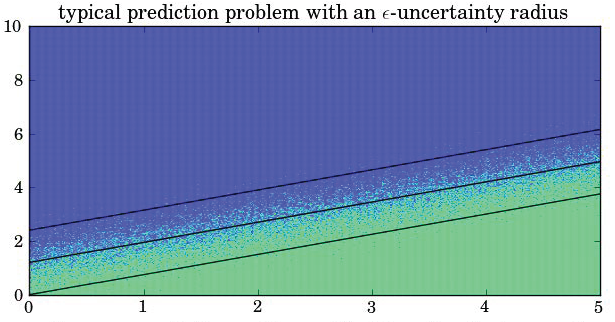
\includegraphics[width=0.49\columnwidth]{plots/example_function_2a.png}
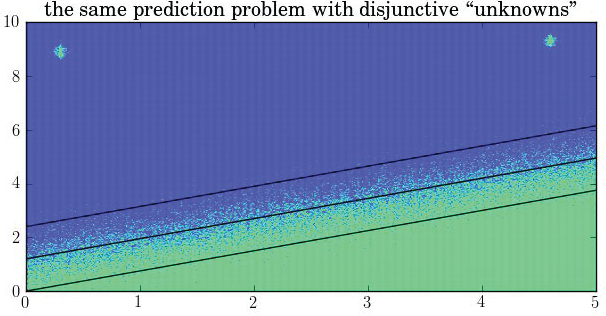
\includegraphics[width=0.49\columnwidth]{plots/example_function_2b.png}
\end{center}
\caption{A typical classification setting. On the the top we see the decision boundary that minimizes the prediction prediction error of a inseparable training set. Additionally, we see the $\epsilon$-radius around the classifier where mistakes are though to occur. The bottom, we see the same classifier with the inclusion of small, disjunctive ``unknowns'', presenting mistakes that occur well outside a model's region of uncertainty. }
\label{fig:unknown}
\end{figure}

Finally, from Figure~\ref{fig:quadrant}, we can see that there is one more type of example: the ``\emph{unknown knowns}''. These are the cases where the model is incorrectly pessimistic: The model reports low confidence and high estimated cost for the examples in these region(s). However, in reality the model generates mostly correct predictions. Such cases are typically easier to manage but may still cause problems in the stakeholders: if this region generates many rejects (with an associated inspection and intervention costs), then the model will be perceived as being overly cautious and potentially inefficient. Despite the fact that it is a promising direction, identifying and dealing with cases of unknown knowns is beyond the scope of this paper, and we leave their study for future work.